\documentclass[12pt]{standalone}
\usepackage{tikz-feynman}

\begin{document}
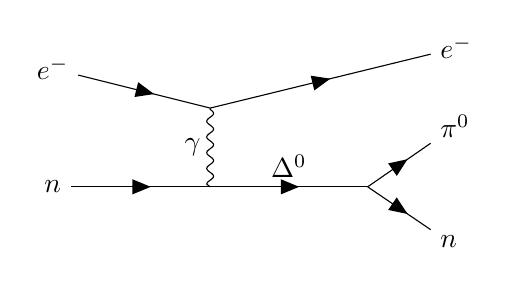
\begin{tikzpicture}
    \begin{feynman}
        \vertex (e1) {$e^-$};
        \vertex [below right=5mm and 20mm of e1] (e2);
        \vertex [above right=5mm and 28mm of e2] (e3) {$e^-$};
        \vertex [below=of e1] (hitnuc1) {$n$};
        \vertex [right=20mm of hitnuc1] (hitnuc2);
        \vertex [right=20mm of hitnuc2] (hitnuc3);
        \vertex [above right=5mm and 8mm of hitnuc3] (dec1) {$\pi^0$};
        \vertex [below right=5mm and 8mm of hitnuc3] (dec2) {$n$};

        \diagram* {
            (e1) -- [fermion] (e2) -- [fermion] (e3),
            (e2) -- [boson, edge label'=\(\gamma\)] (hitnuc2),
            (hitnuc1) -- [fermion] (hitnuc2) -- [fermion, edge label=\(\Delta^{0}\)] (hitnuc3),
            (hitnuc3) -- [fermion] (dec1),
            (hitnuc3) -- [fermion] (dec2),
        };
    \end{feynman}
\end{tikzpicture}

\end{document}
